\begin{figure*}%[!h]
\center
% \begin{tabular}{c|c|c|c}
\definecolor{darkgreen}{rgb}{0, 0.5, 0}
\newcommand{\bluetri}{{\color{blue} $\blacktriangle$}}
\newcommand{\greentri}{{\color{darkgreen} $\blacktriangle$}}
\newcommand{\redtri}{{\color{red} $\blacktriangle$}}
\newcommand{\bluecir}{{\color{blue} $\circ$}}
\newcommand{\greencir}{{\color{darkgreen} $\circ$}}
\newcommand{\redcir}{{\color{red} $\circ$}}
\begin{tabular}{ccc}
\hspace{-7cm}\panel{A} & \hspace{-2cm}\panel{C} & \hspace{-3.5cm}\panel{D}\\[-1cm]
\raisebox{10.7cm}{\hspace{-0.2cm}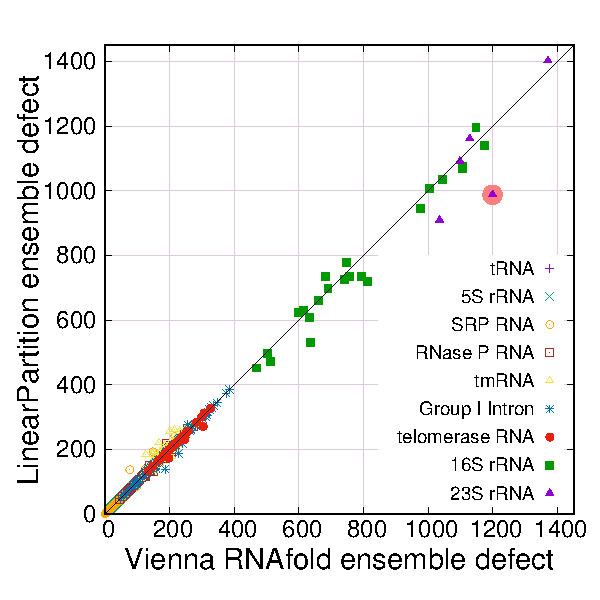
\includegraphics[width=0.4\textwidth]{figs/ensemble_defect}} &
% \hspace{-.2cm}\panel{A} & \hspace{-0.6cm}\panel{B} \\[-1cm] %& \hspace{-2.5cm}\panel{D}
	\multicolumn{2}{c}{
	  \hspace{-.7cm}
	  \raisebox{12.4cm}{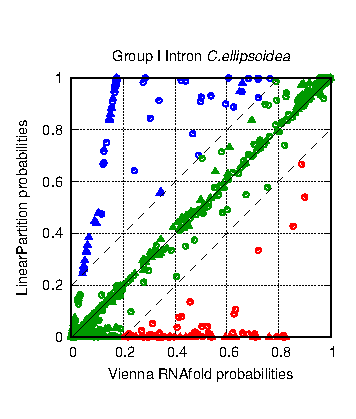
\includegraphics[width=5.2cm]{figs/prob_xy_grp1}}
	  \hspace{-5.1cm}
	  \raisebox{4cm}{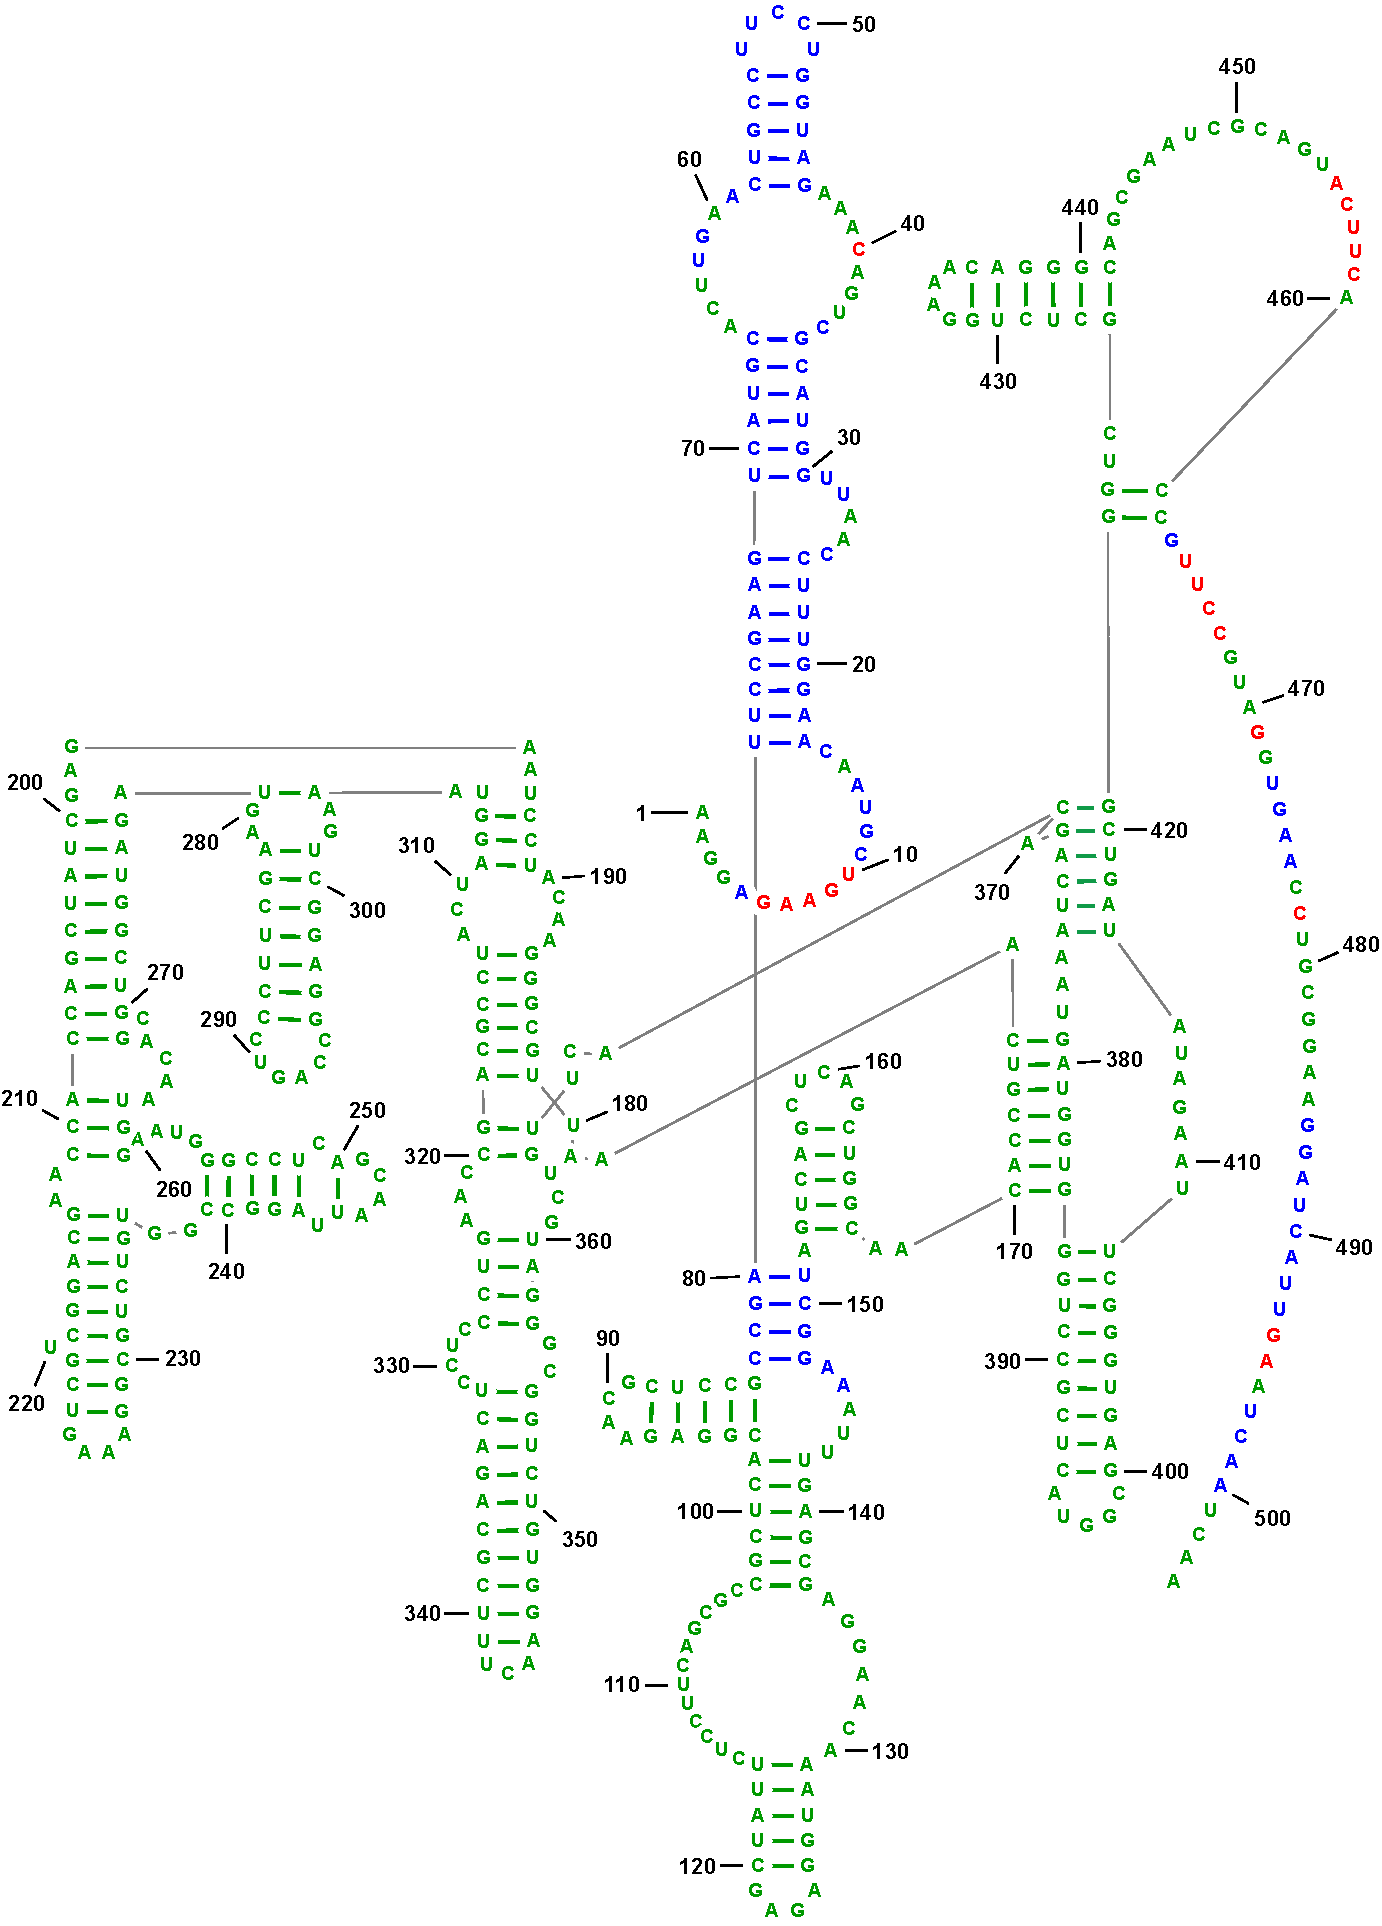
\includegraphics[width=0.58\textwidth]{figs/grp1_70_gutell_modified_2020}}
  	} \\[-11cm]
\hspace{-7cm}\panel{B} &\\[-.5cm]
\raisebox{.cm}{\hspace{-0.2cm}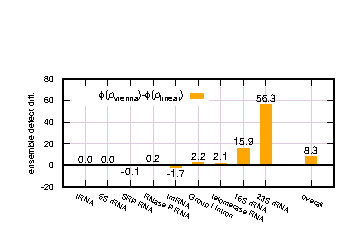
\includegraphics[width=0.42\textwidth]{figs/ensemble_defect_histogram}} & \\[-.4cm]
% \hspace{-.2cm}\raisebox{1cm}{\panel{C}} & \\[-1cm]
\hspace{-7cm}\panel{E} &\\[-.5cm]
\multicolumn{2}{l}{% \hspace{-0.3cm}
\resizebox{0.58\textwidth}{!}{
  \begin{tabular}{cr@{\; }r@{\quad \quad}r@{\; }r}
%	\toprule
         &     \multicolumn{2}{c}{total} & \multicolumn{2}{c}{correct} \\
			 \midrule
{\color{blue} $p_\linear \!-\! p_\vienna \!>\! 0.2$} & 55 \bluetri & 40 \bluecir  & 23 \bluetri & 37 \bluecir \\
{\color{darkgreen} $|p_\linear \!-\! p_\vienna| \!\leq \!0.2$} &  126,645 \greentri & 420 \greencir & 111 \greentri & 180 \greencir\\
{\color{red} $p_\linear \!-\! p_\vienna \!<\! -0.2$} & 56 \redtri & 44 \redcir & 0 \redtri & 19 \redcir \\[1.9cm]
%	                 \bottomrule
  \end{tabular}}
}
\end{tabular}\\[-2cm]
\begin{tabular}{cccc}
\hspace{-4.4cm} \panel{F} & \hspace{-4.6cm}\panel{G} & \hspace{-4.6cm}\panel{H} & \hspace{-4.6cm}\panel{I}\\[-0.2cm]
\hspace{-0.2cm}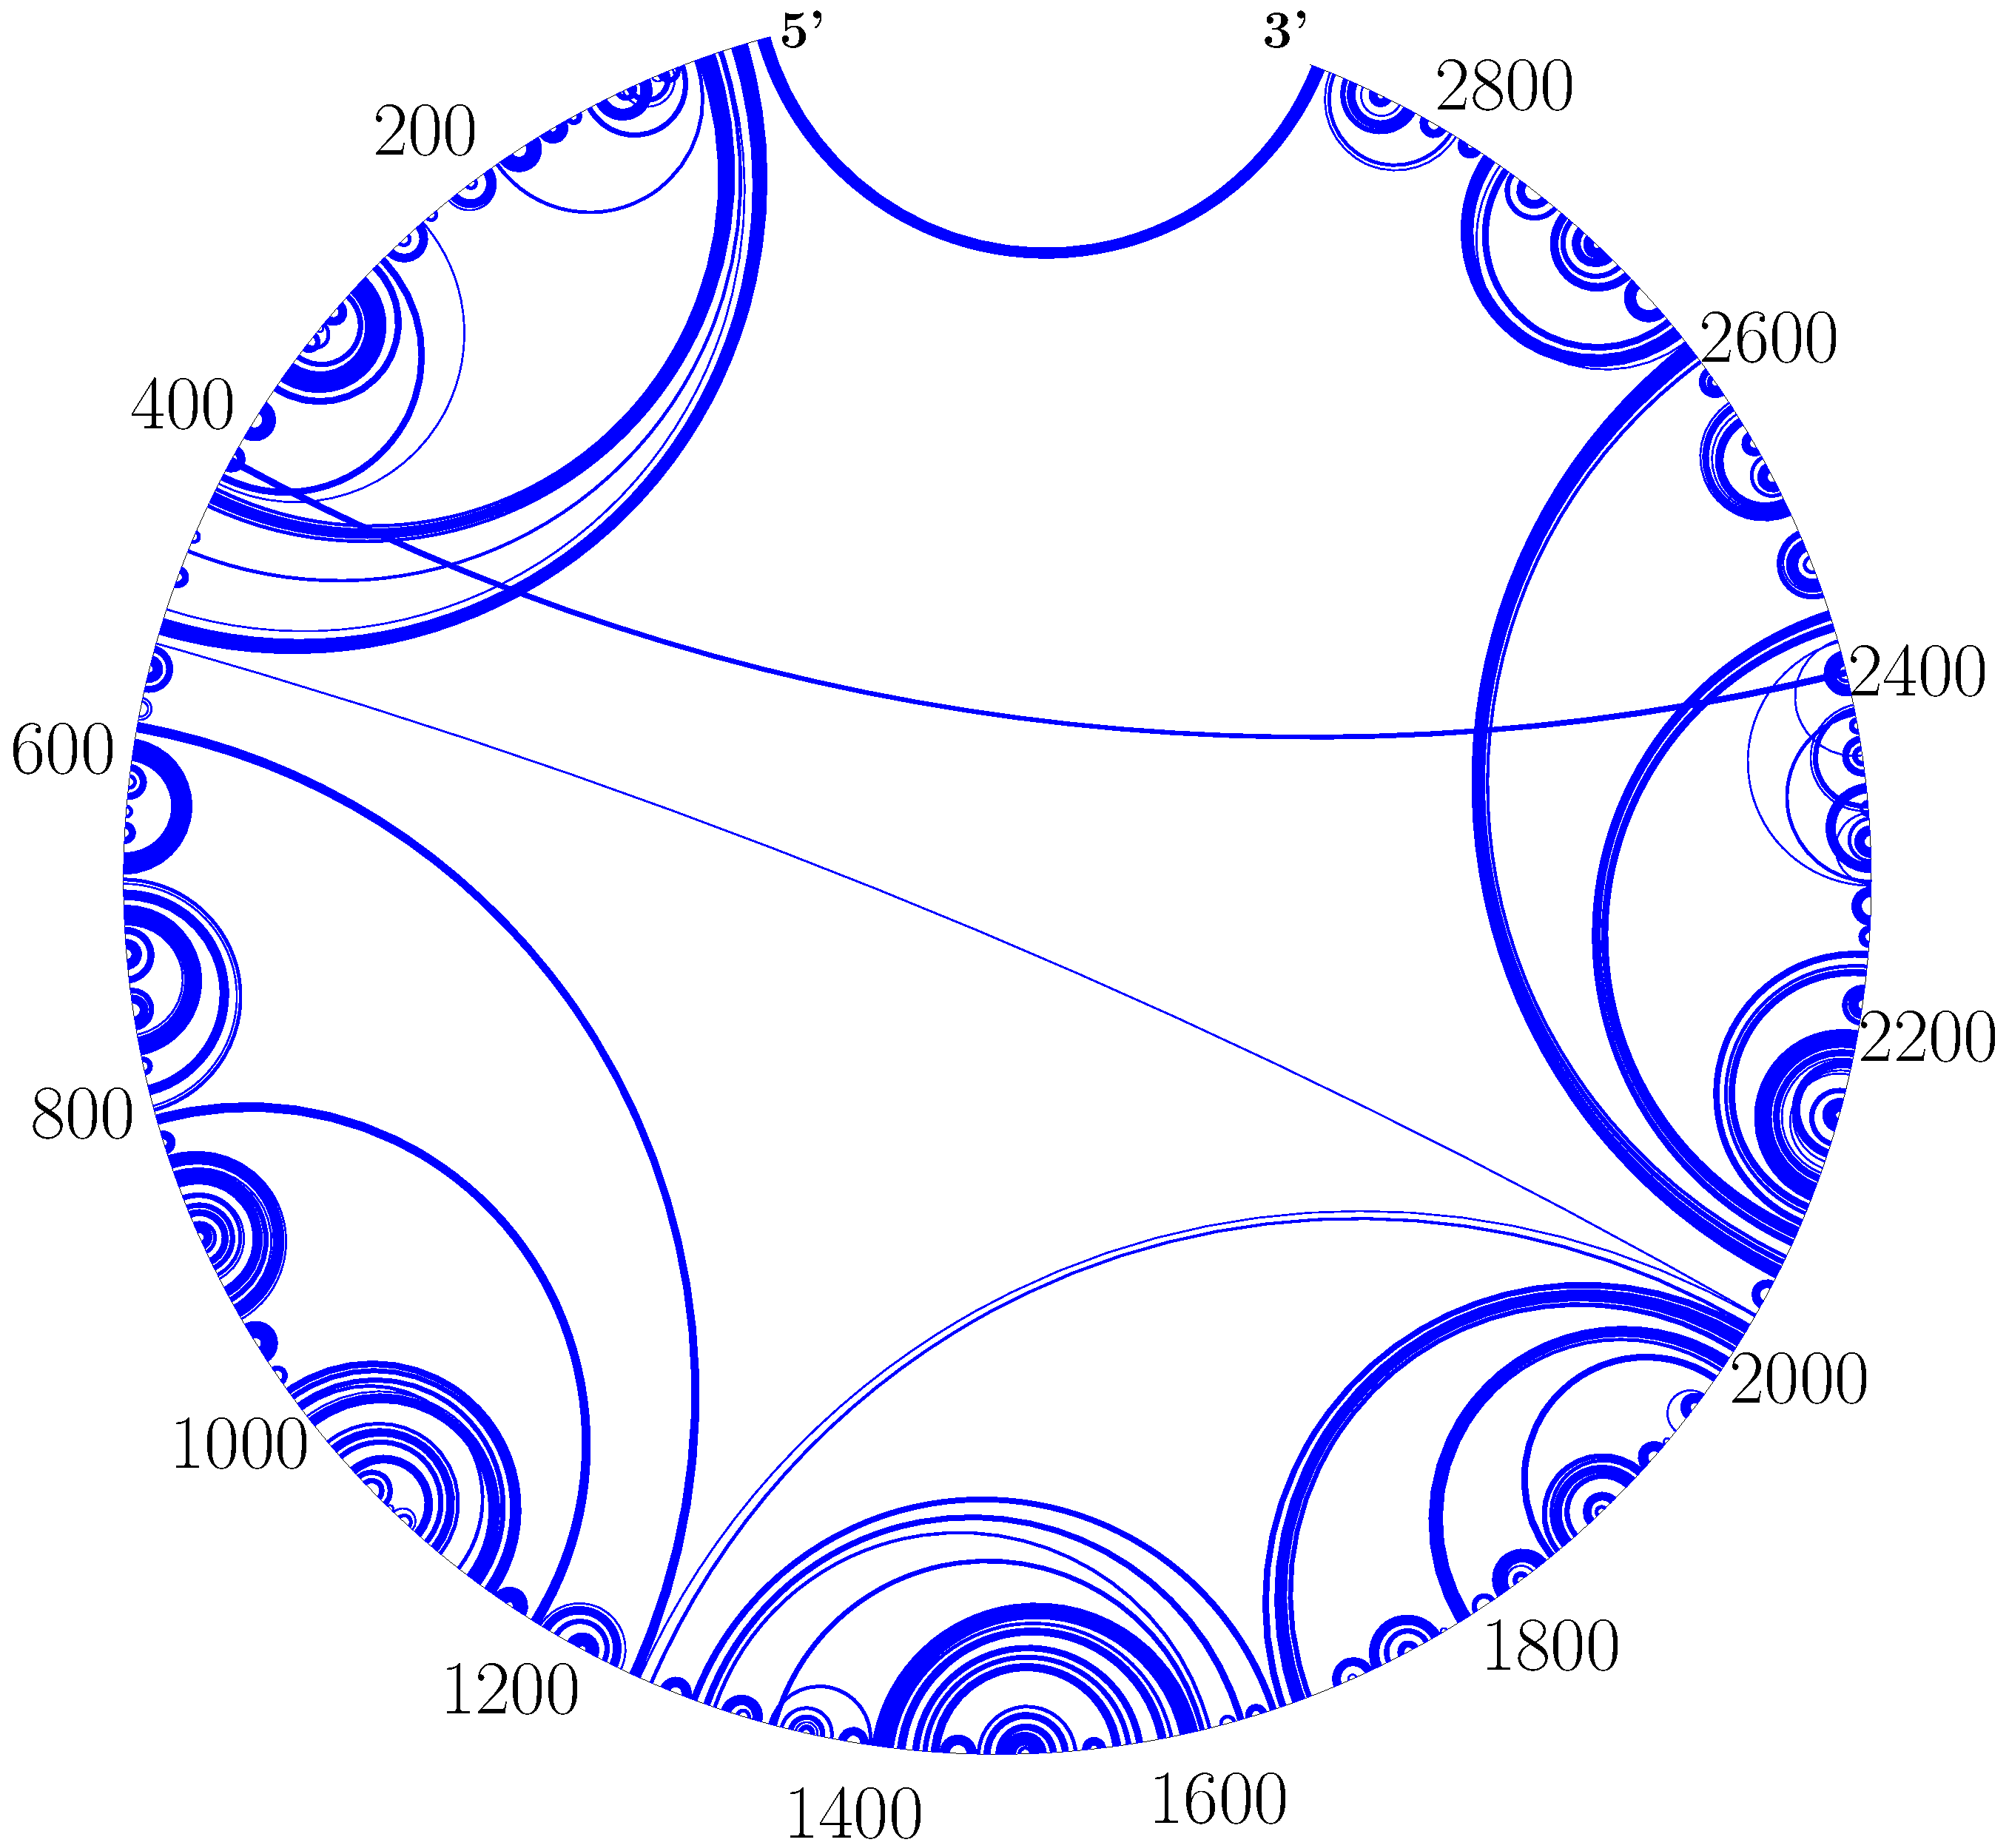
\includegraphics[width=0.25\textwidth]{figs/23s_gold} &
\hspace{-0.35cm}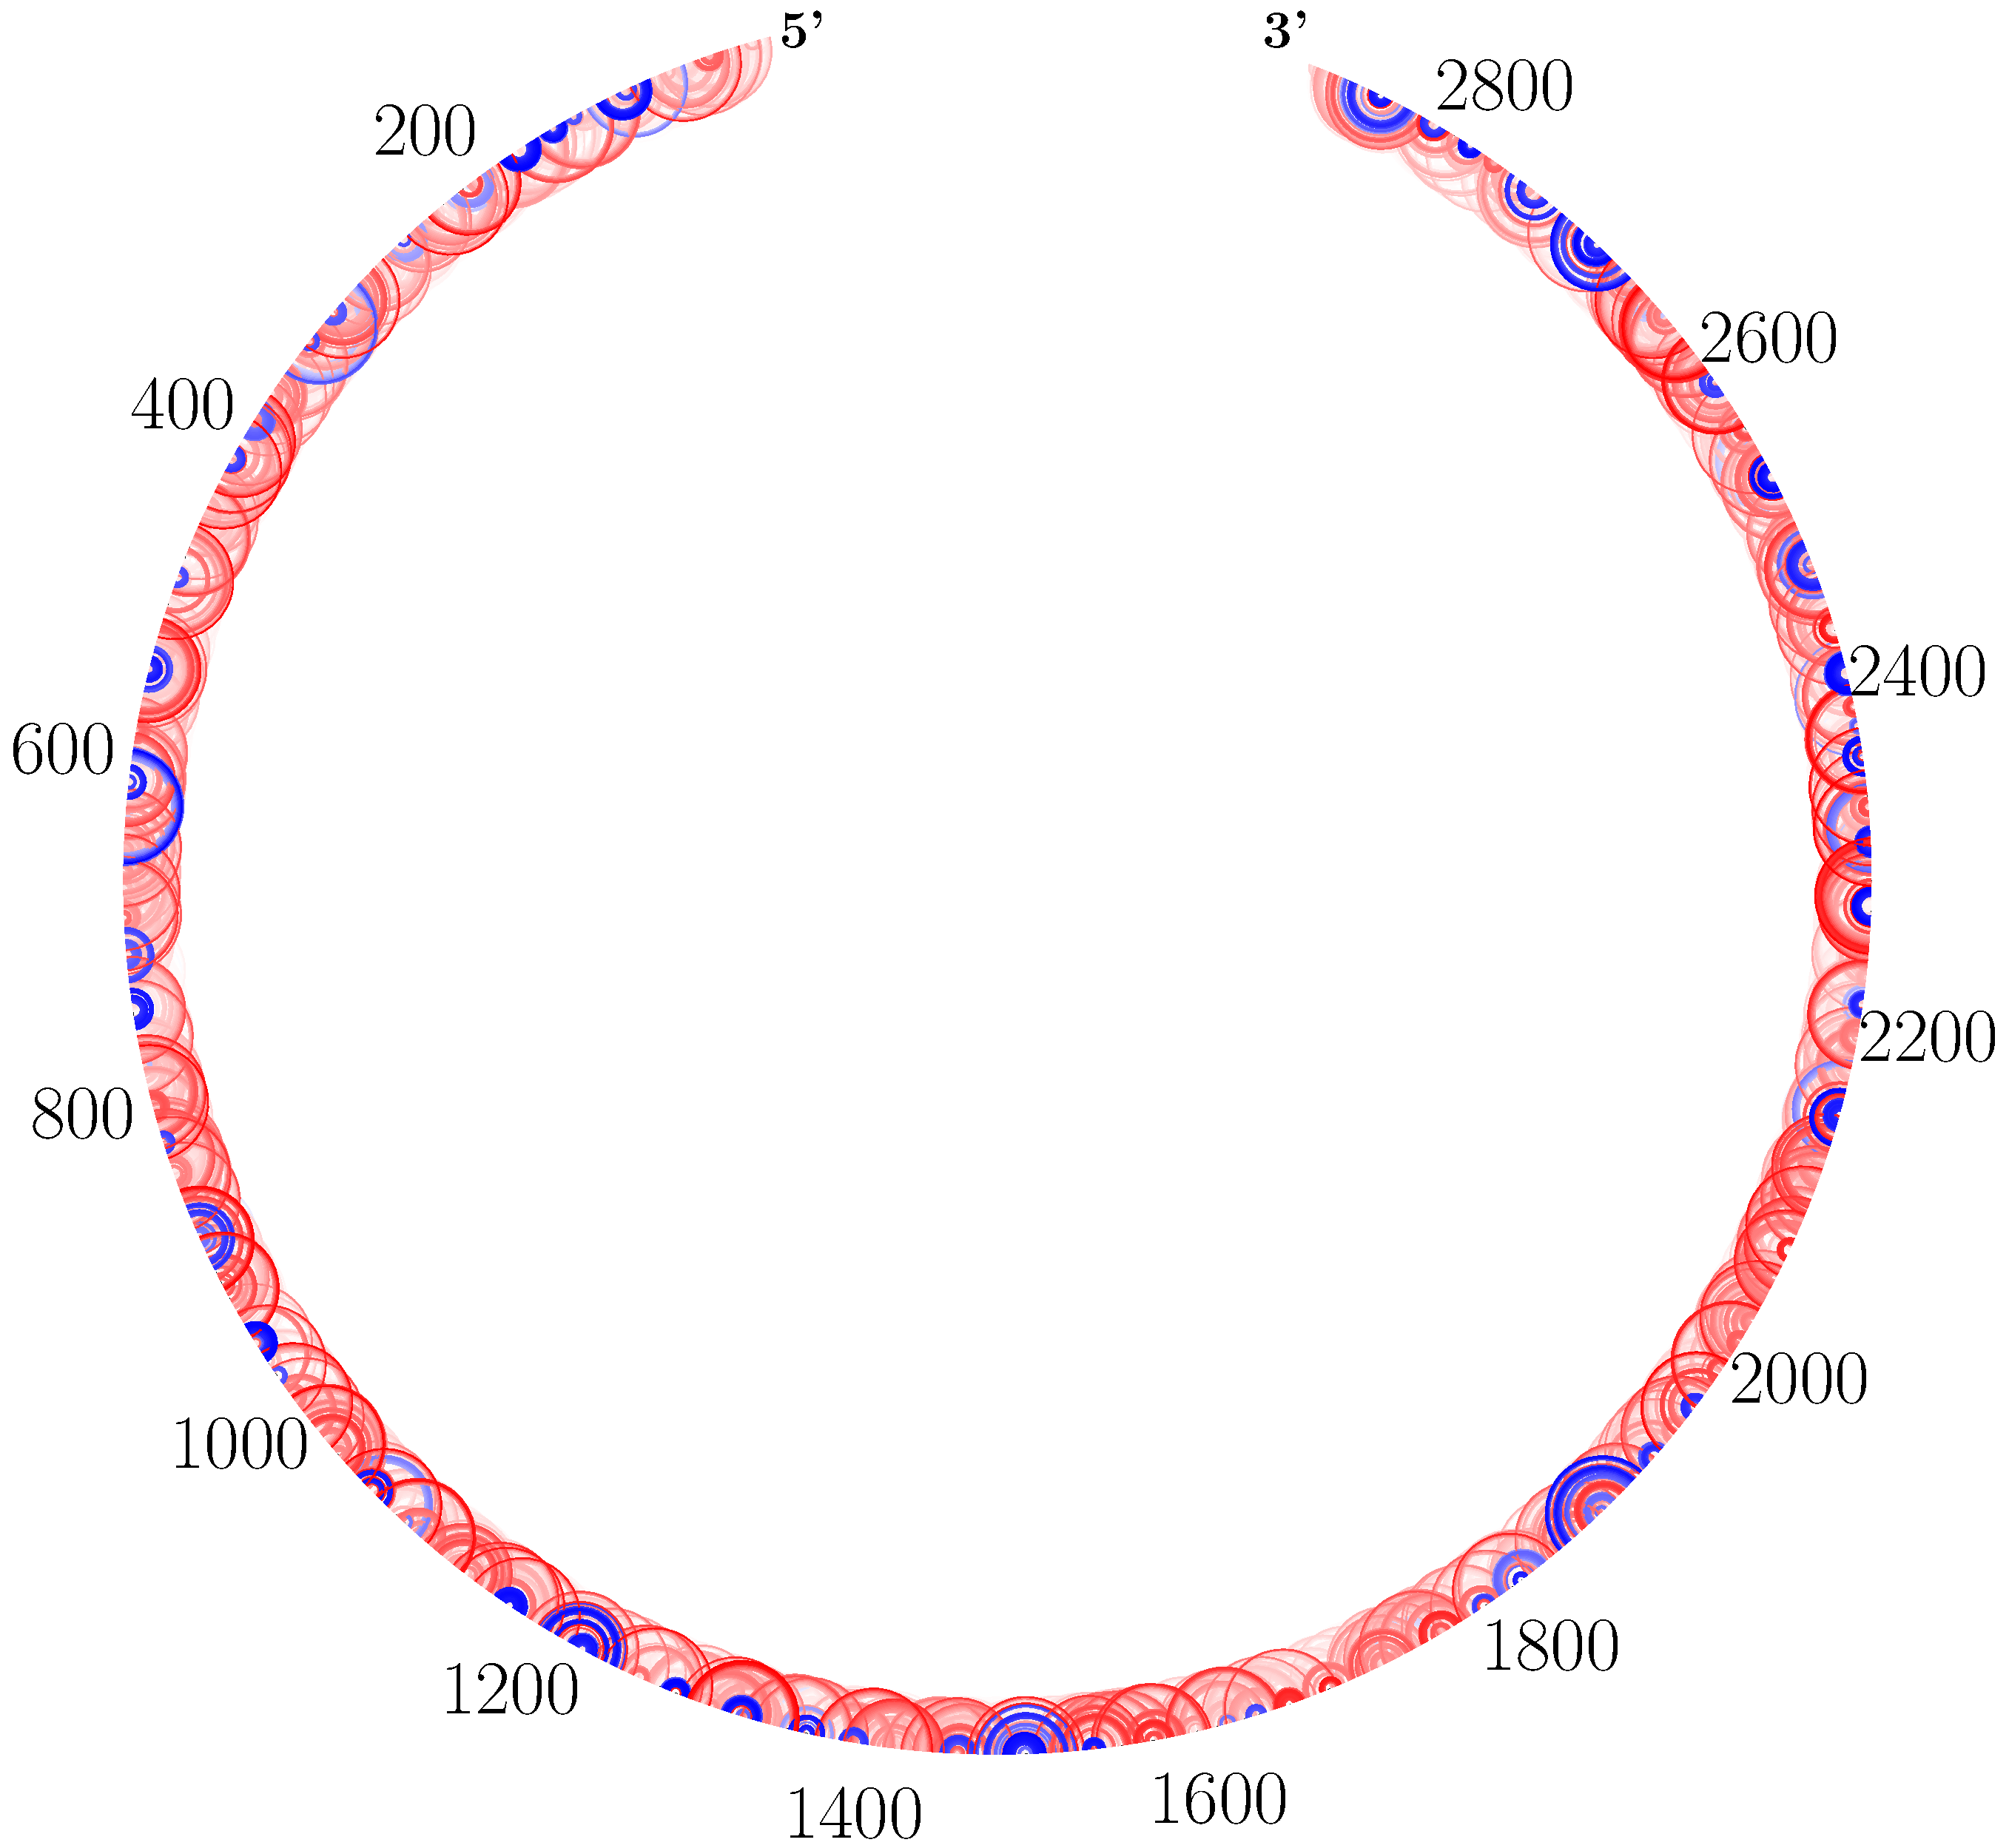
\includegraphics[width=0.25\textwidth]{figs/23s_vienna_plfold_example.pdf} &
\hspace{-0.35cm}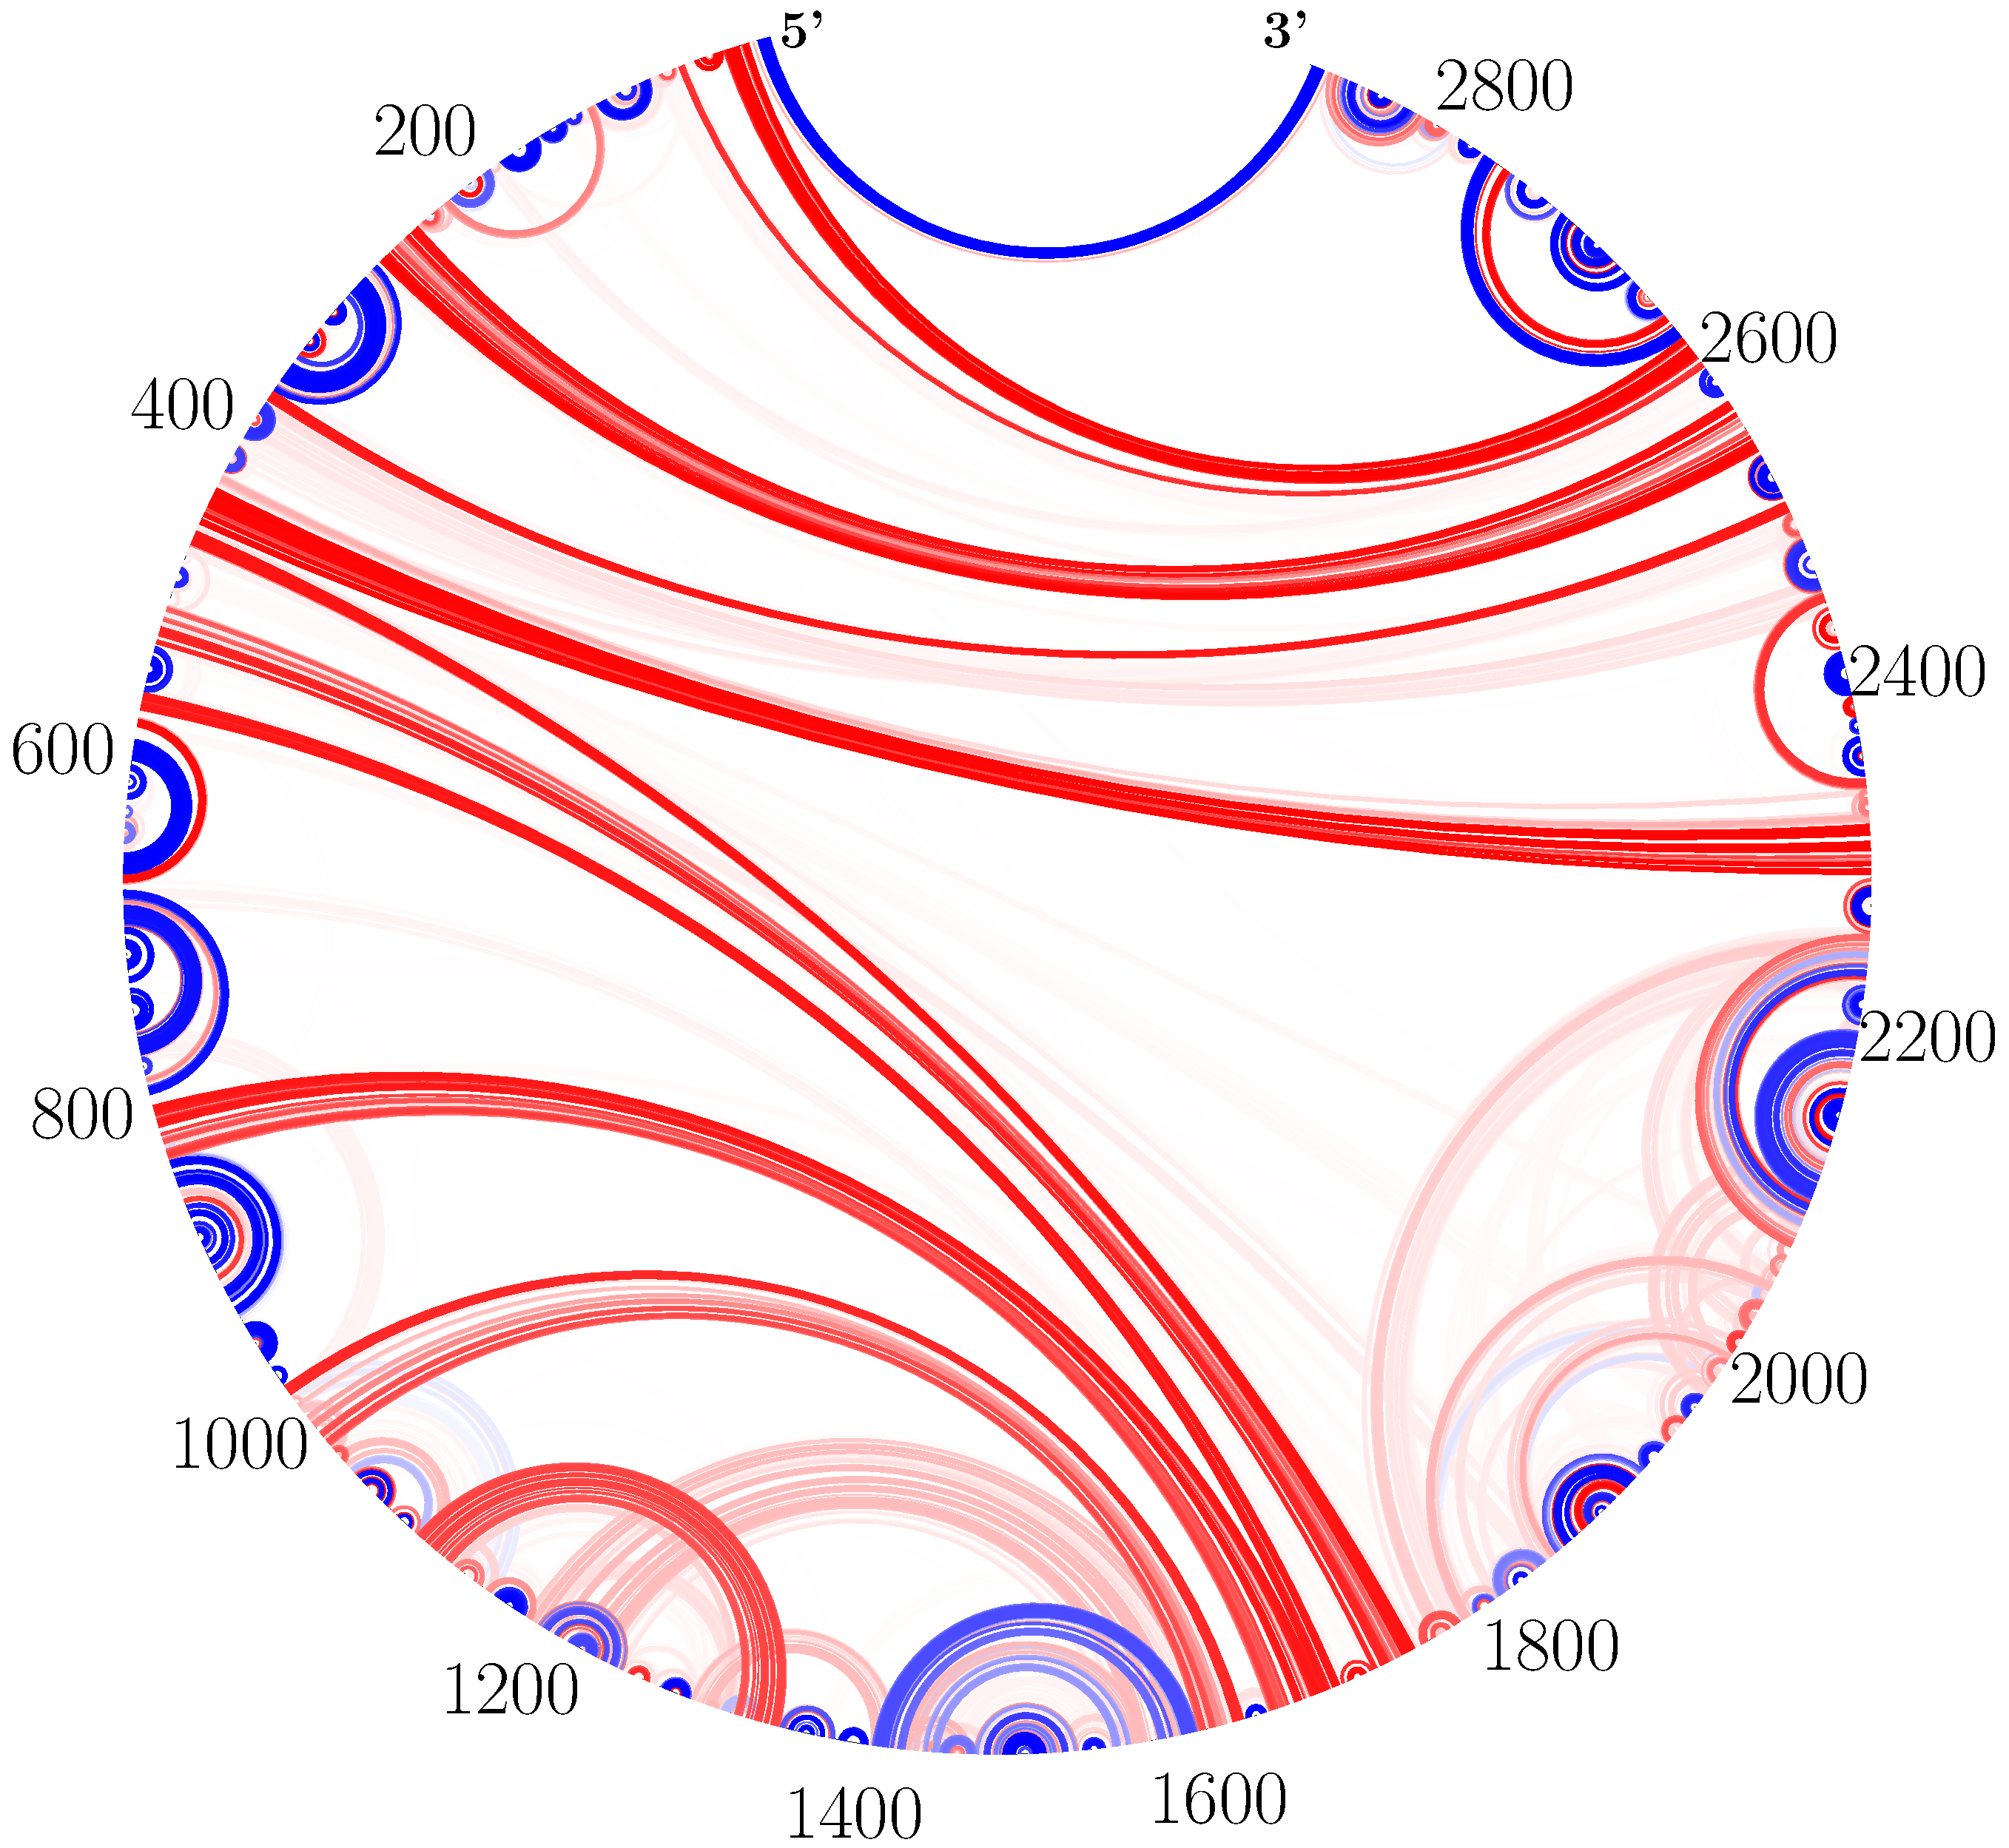
\includegraphics[width=0.25\textwidth]{figs/23s_vienna_example} &
\hspace{-0.35cm}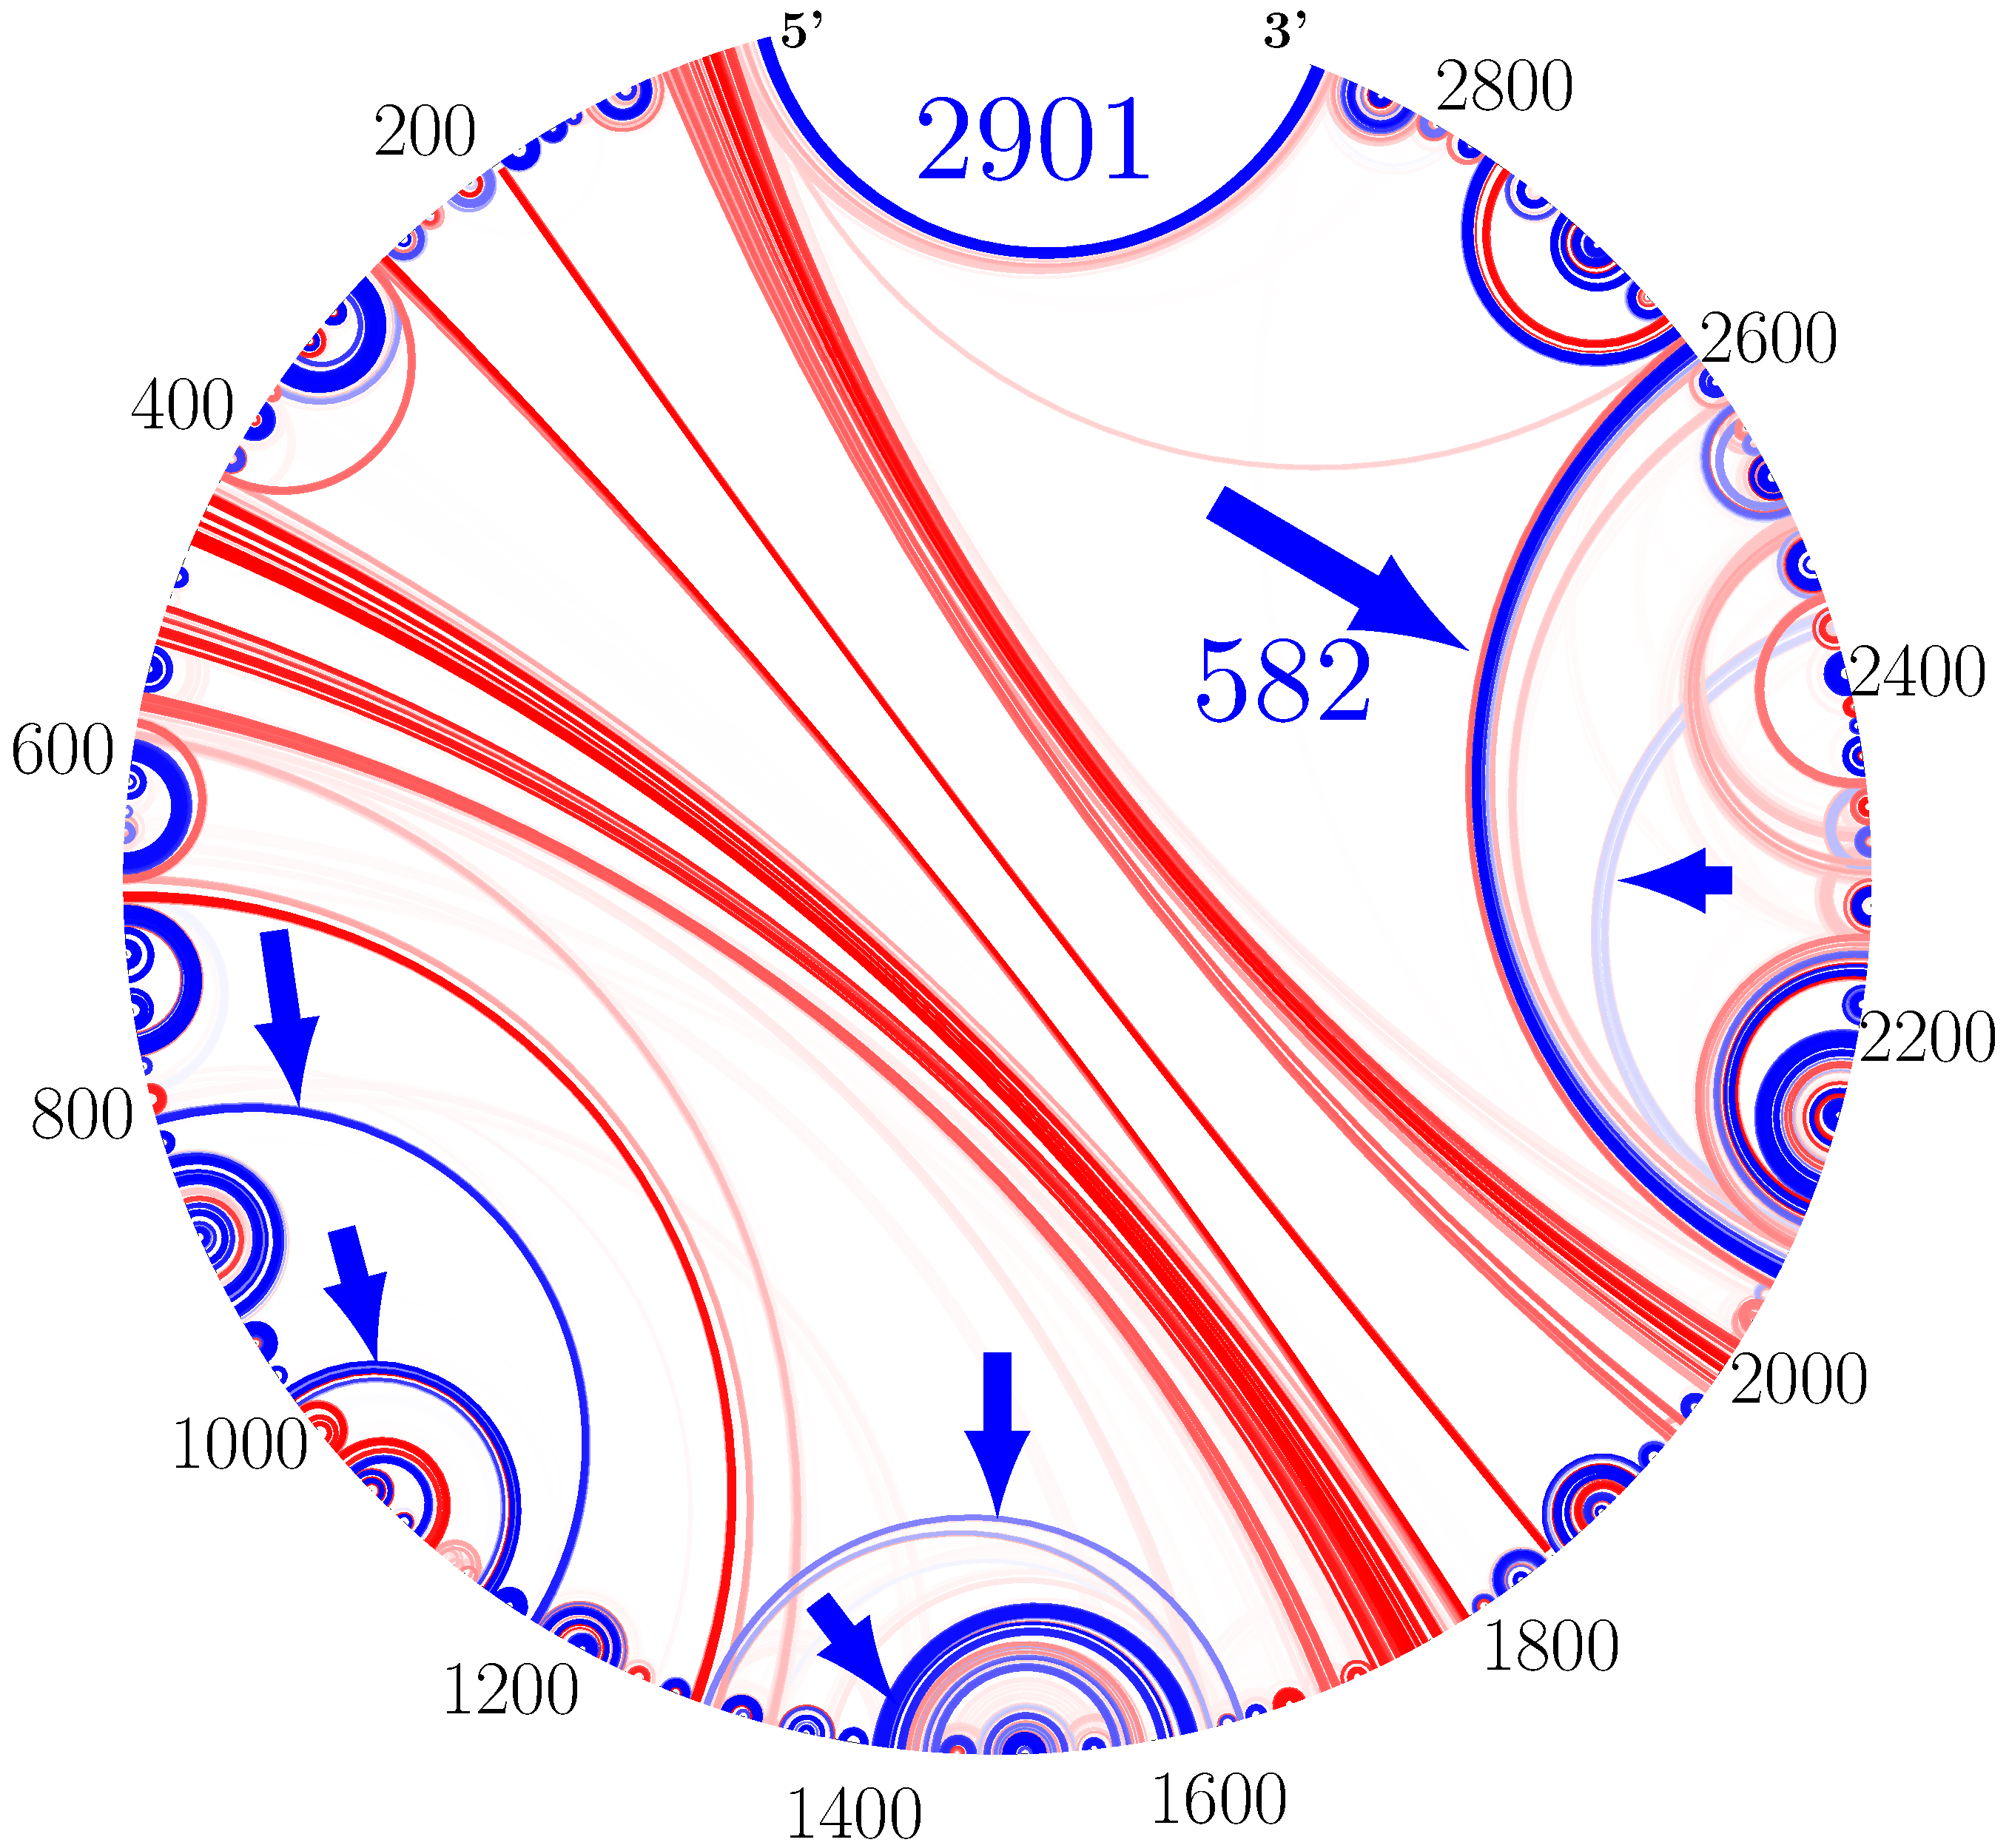
\includegraphics[width=0.25\textwidth]{figs/23s_example.pdf}
\end{tabular}
\caption{
{\bf A}: Ensemble defect comparison between \viennarnafold and \linearpartition on the ArchiveII dataset.
{\bf B}: Ensemble defect difference for each family.
{\bf C--E}: An example of {\it C.~ellipsoidea} Group I Intron. 
{\bf C}: solid triangles ({\small {\color{blue} $\blacktriangle$} {\color{darkgreen}$\blacktriangle$}  {\color{red}$\blacktriangle$}}) stand for base pairing probabilities and
unfilled circles ({\small {\color{blue} $\circ$} {\color{darkgreen}$\circ$}  {\color{red}$\circ$}})  stand for single-stranded probabilities.
{\color{blue} blue: $p_\linear \!-\! p_\vienna \!>\! 0.2$};
{\color{darkgreen} green: $|p_\linear \!-\! p_\vienna| \!\leq \!0.2$};
{\color{red} red: $p_\linear \!-\! p_\vienna \!<\! -0.2$};
%some high probability pairs and unpaired bases in \linearpartition have low probabilities in \viennarnafold (in blue), and some low probability ones in \linearpartition have high probabilities in \viennarnafold (in red); 
	{\bf D}: ground truth structure colored with the above scheme; % from \viennarnafold and \linearpartition; 
	%pink binds around position 370 are pseudoknotted pairs.
	{\bf E}: statistics of this example. 
	"total" columns are the total numbers of triangles and circles with different colors in {\bf A},
	while "correct" columns are the corresponding numbers %of such triangles and circles
        in the ground-truth structure  in {\bf B},
        which is better correlated with \linearpartition's probabilities than \viennarnafold's ({\color{blue} 23 blue pairs} and {\color{red} 0 red pairs}). %ground-truth structure.
	% Note that each triangle represents a pair of nucleotides.
{\bf F--I}: An example of \ecoli 23S rRNA. 
	{\bf F}: circular plot of the ground truth.
{\bf G-I}: circular plots using the base pair probabilities from \viennarnaplfold (with default window size $70$), \rnafold and \linearpartition, respectively; 
base pairs in the ground truth are in blue;
the color shade of the lines are propotional to their probabilities.
	\label{example}\\[-.7cm]
}
\end{figure*}
